\documentclass[portait]{article}

\usepackage[T1]{fontenc}
\usepackage{indentfirst}
\usepackage{algorithm2e}
\usepackage{xcolor,graphicx,url}
\usepackage[utf8]{inputenc}
\usepackage{subfigure}
\usepackage{amsmath}
\usepackage{newcent} 
\usepackage{palatino, url, multicol}
\usepackage{listings}
\usepackage{lscape}
\usepackage{synttree}
\usepackage{pdfpages}
\usepackage{paralist}
\usepackage{subfigure}

\usepackage[margin=.5in, textwidth=500pt]{geometry}


%\usepackage[table]{xcolor}% http://ctan.org/pkg/xcolor

\usepackage{xcolor,colortbl}
%\definecolor{green}{rgb}{0.1,0.1,0.1}
\newcommand{\done}{\cellcolor{teal}done}  %{0.9}
\newcommand{\hcyan}[1]{{\color{teal} #1}}




\author{}
\date{}
\setlength{\topmargin}{-0.9in}
\setlength{\textheight}{23cm}
\setlength{\oddsidemargin}{-6mm}
\setlength{\textwidth}{7in} 

\begin{document}
%\maketitle


\everymath{\displaystyle}


%This experiment consists of a matrix transposition execution 


\begin{algorithm}[H]
   fill a matrix $m_{n,n}$ with random values\;
   sleep during $t$ seconds\;
   transpose the matrix $m$ \:
\end{algorithm}

\footnotesize
\begin{figure}[htb]%
  \centering
   \vspace{-8pt}
   \centering
         \subfigure{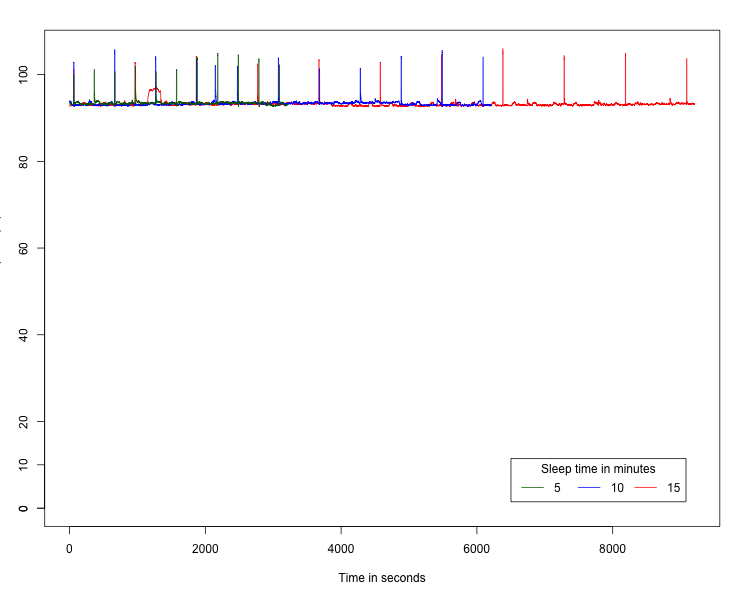
\includegraphics[width=3.0in]{results/external-loop/2013-06-24_13-53/10/1600000/10000/10000.png}}    
	\subfigure{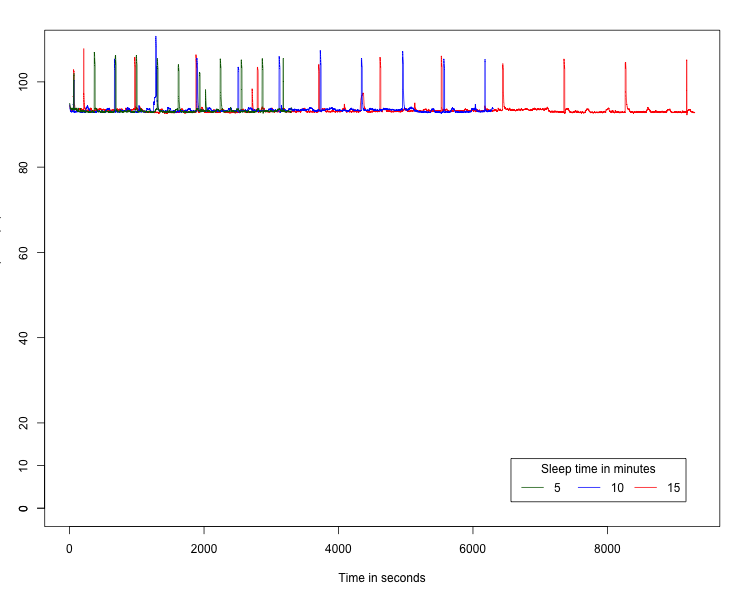
\includegraphics[width=3.0in]{results/external-loop/2013-06-24_13-53/10/1600000/20000/20000.png}}  	
	\subfigure{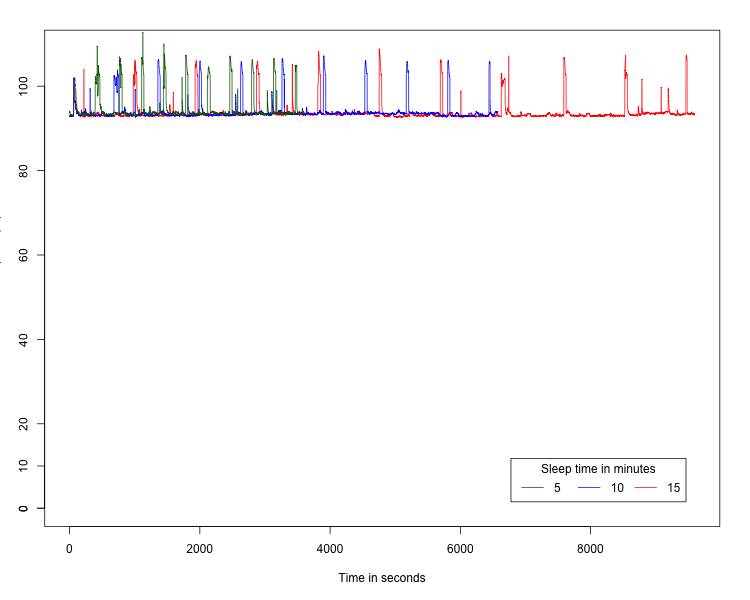
\includegraphics[width=3.0in]{results/external-loop/2013-06-24_13-53/10/1600000/30000/30000.png}}
   \vspace{-8pt}	
\caption{Power consumption of a square matrix transposition, CPU frequency of 1.6 GHz, and matrix size of (a) 10,000 (b) 20,000 and (c) 30,000} 
\end{figure}
\normalsize


\footnotesize
\begin{figure}[htb]%
  \centering
   \vspace{-8pt}
   \centering
         \subfigure{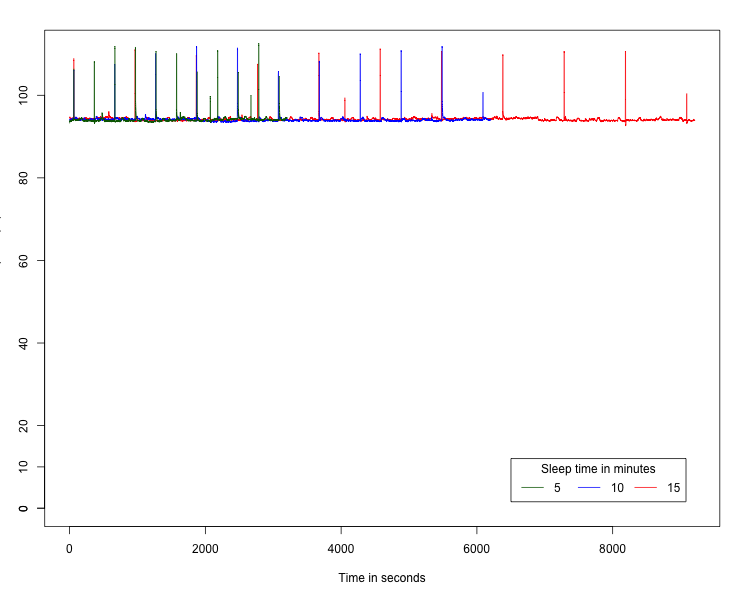
\includegraphics[width=3.0in]{results/external-loop/2013-06-24_13-53/10/1867000/10000/10000.png}}    
	\subfigure{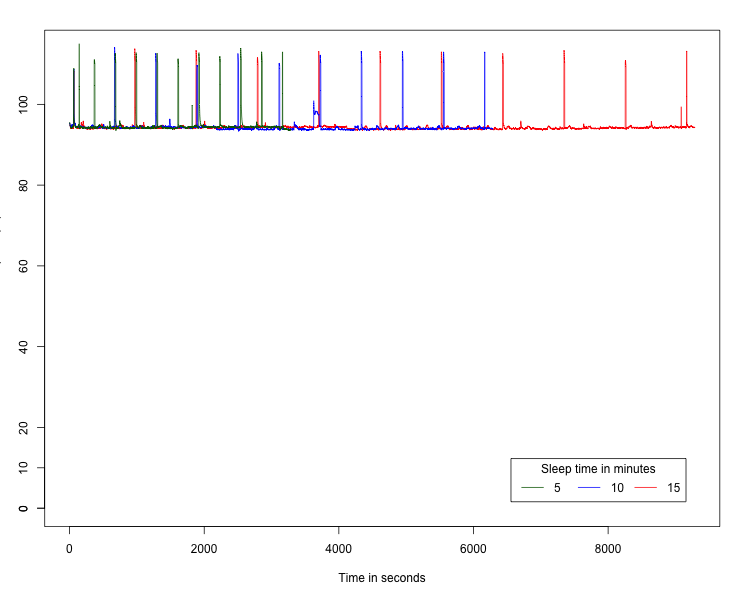
\includegraphics[width=3.0in]{results/external-loop/2013-06-24_13-53/10/1867000/20000/20000.png}}  	
	\subfigure{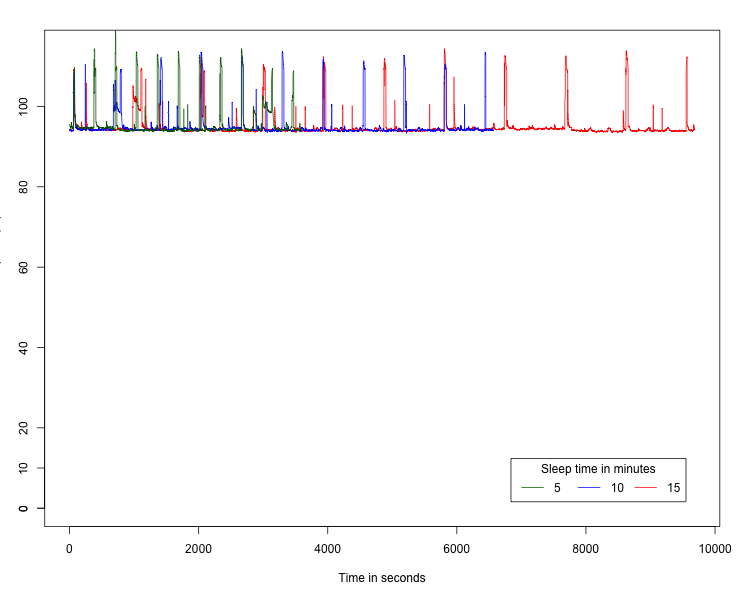
\includegraphics[width=3.0in]{results/external-loop/2013-06-24_13-53/10/1867000/30000/30000.png}}
   \vspace{-8pt}	
\caption{Power consumption of a square matrix transposition, CPU frequency of 1.86 GHz, and matrix size of (a) 10,000 (b) 20,000 and (c) 30,000} 
\end{figure}
\normalsize

\footnotesize
\begin{figure}[htb]%
  \centering
   \vspace{-8pt}
   \centering
         \subfigure{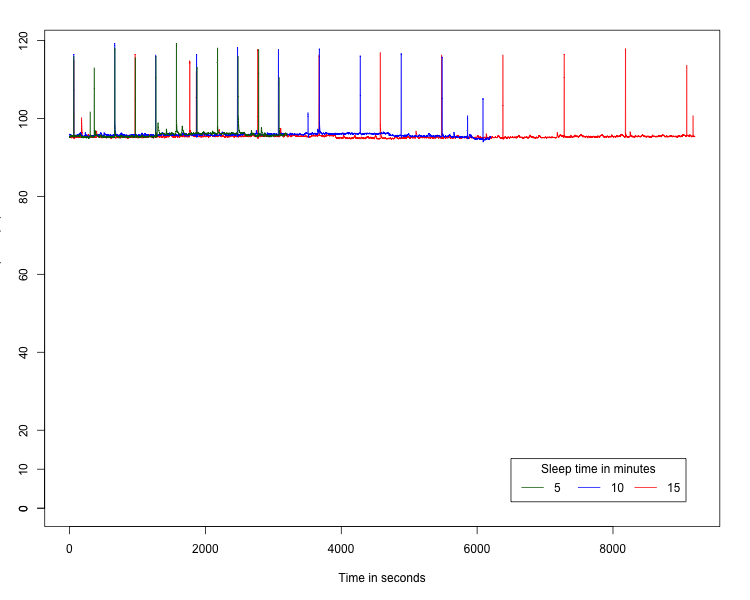
\includegraphics[width=3.0in]{results/external-loop/2013-06-24_13-53/10/2133000/10000/10000.png}}    
	\subfigure{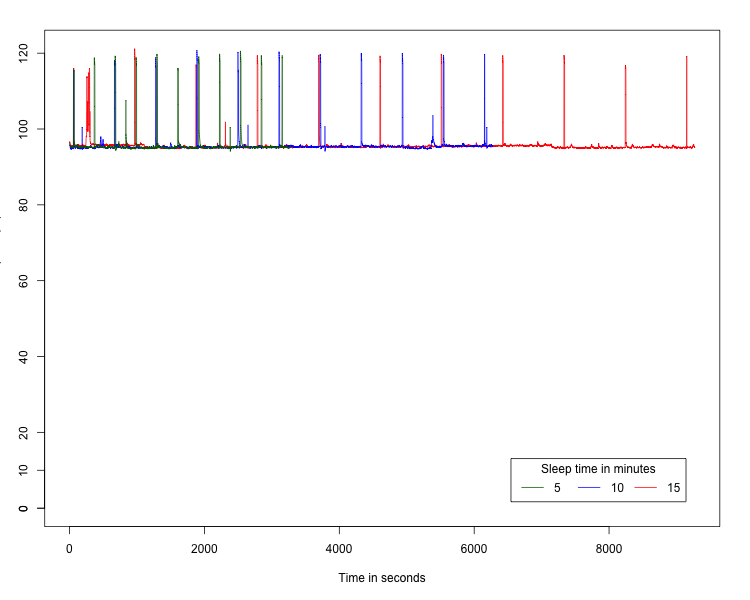
\includegraphics[width=3.0in]{results/external-loop/2013-06-24_13-53/10/2133000/20000/20000.png}}  	
	\subfigure{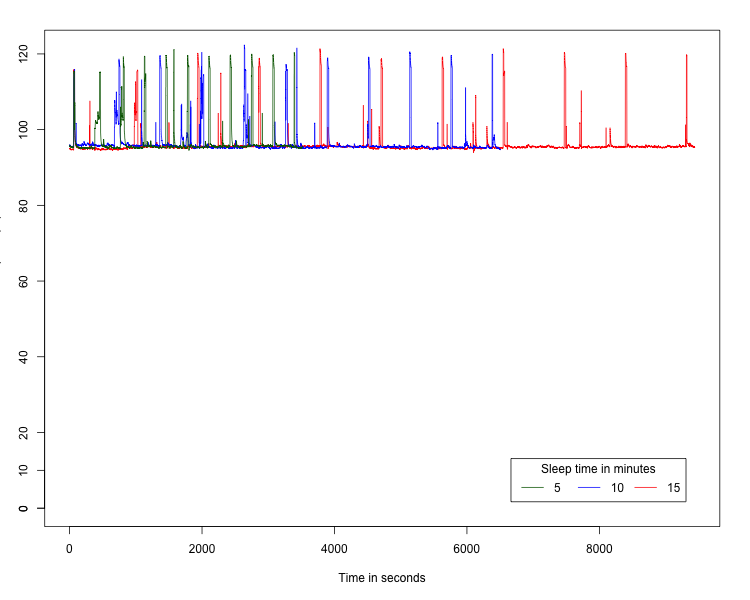
\includegraphics[width=3.0in]{results/external-loop/2013-06-24_13-53/10/2133000/30000/30000.png}}
   \vspace{-8pt}	
\caption{Power consumption of a square matrix transposition, CPU frequency of 2.13 GHz, and matrix size of (a) 10,000 (b) 20,000 and (c) 30,000} 
\end{figure}
\normalsize

\footnotesize
\begin{figure}[htb]%
  \centering
   \vspace{-8pt}
   \centering
         \subfigure{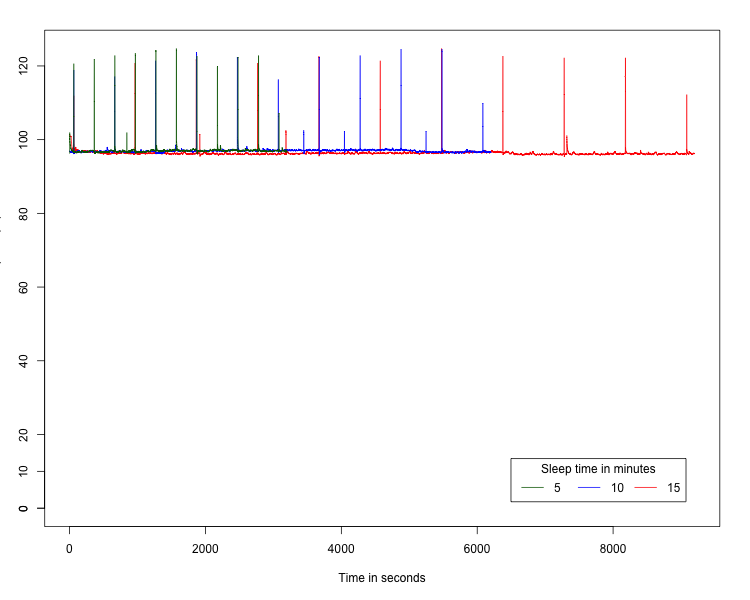
\includegraphics[width=3.0in]{results/external-loop/2013-06-24_13-53/10/2400000/10000/10000.png}}    
	\subfigure{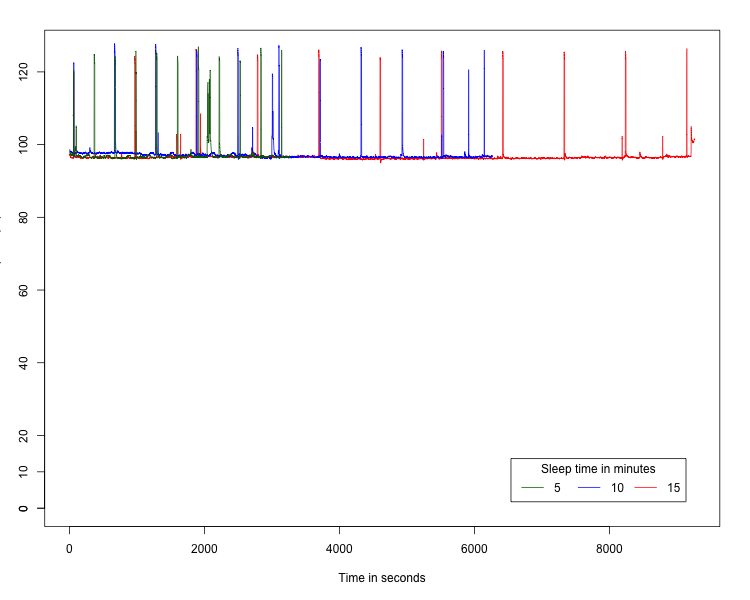
\includegraphics[width=3.0in]{results/external-loop/2013-06-24_13-53/10/2400000/20000/20000.png}}  	
	\subfigure{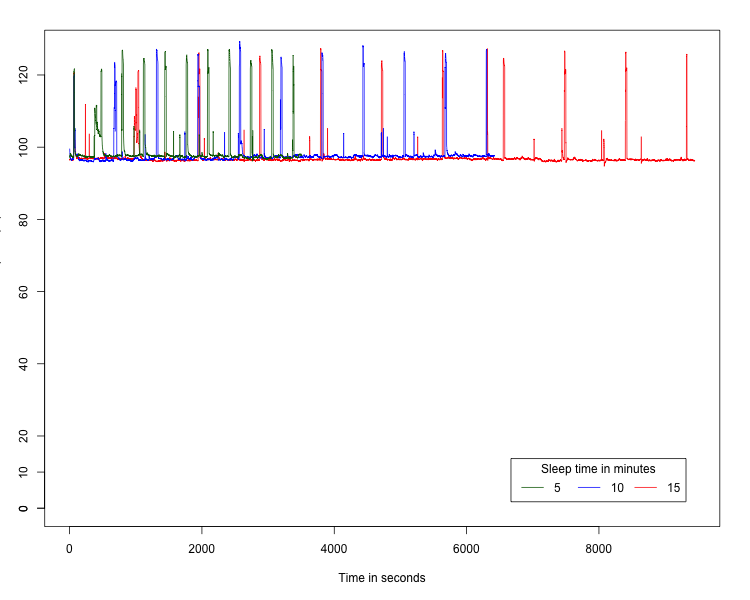
\includegraphics[width=3.0in]{results/external-loop/2013-06-24_13-53/10/2400000/30000/30000.png}}
   \vspace{-8pt}	
\caption{Power consumption of a square matrix transposition, CPU frequency of 2.13 GHz, and matrix size of (a) 10,000 (b) 20,000 and (c) 30,000} 
\end{figure}
\normalsize






\end{document}